\documentclass[10pt]{article}
\usepackage[a4paper,margin=17mm]{geometry}
\usepackage{graphicx,hyperref,booktabs,amsmath}
\hypersetup{colorlinks=true,urlcolor=blue}
\setlength{\parindent}{0pt}\setlength{\parskip}{5pt}
\begin{document}
\begin{center}\Large Bounded leased affine consequences\\[3pt]
\normalsize Preserved completions with unchanged curve search --- 17 November 2026\end{center}
The Rust component borrows the original System and dependency/cache arrays,
then admits bounded linear consequences at propagation quiescence. Separate
direct BigUint arithmetic checks weighted original rows, exact premises and
labelled unit applications; leases disappear before LIFO Undo. Producer native
PCC-20261117-532e0c; all standing unsigned/unverified. [pcc:unverified]

\begin{center}\begin{tabular}{lrrr}\toprule
Fixed curve inputs, $n=28$ & Root & Unsupported & Model cap\\\midrule
Old v1 / exact disabled &15&13&0\\
Earlier broader recompute v1 &13&0&15\\
Bounded leased v1 &15&13&0\\\bottomrule
\end{tabular}\end{center}
No baseline completion is lost; no completed-curve node gain is recorded.
The new mechanism is narrower than the earlier enabled arm: it uses an
incomplete affine slice, with no nonlinear rewriting or quadratic-row
cancellation. Zero caps is not an equivalent-engine speed/cost result.
The 64 MiB ceiling measures cumulative modeled reservations, not live memory
or RSS. Caps and Unsupported are not absence certificates. [pcc:unverified]

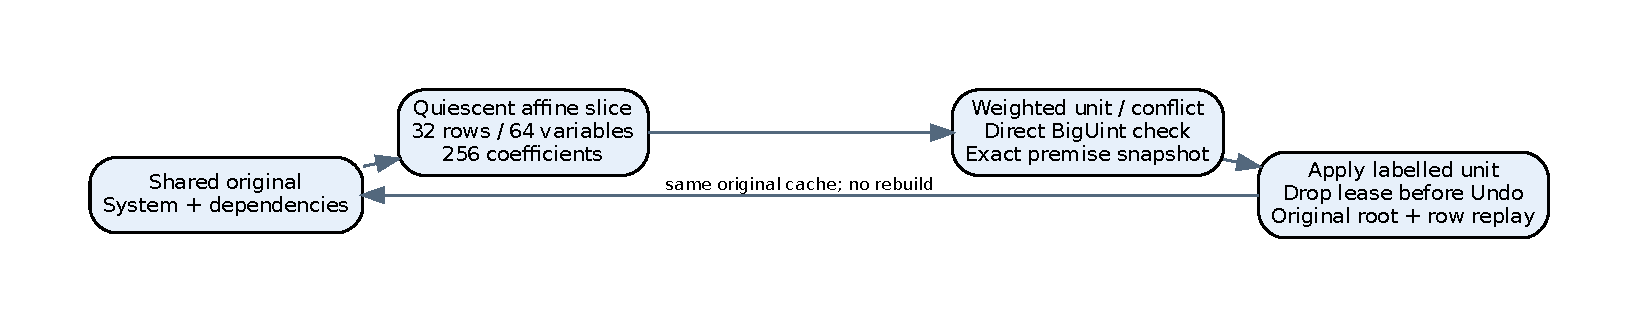
\includegraphics[width=\linewidth,height=34mm,keepaspectratio]{pipeline.pdf}\par
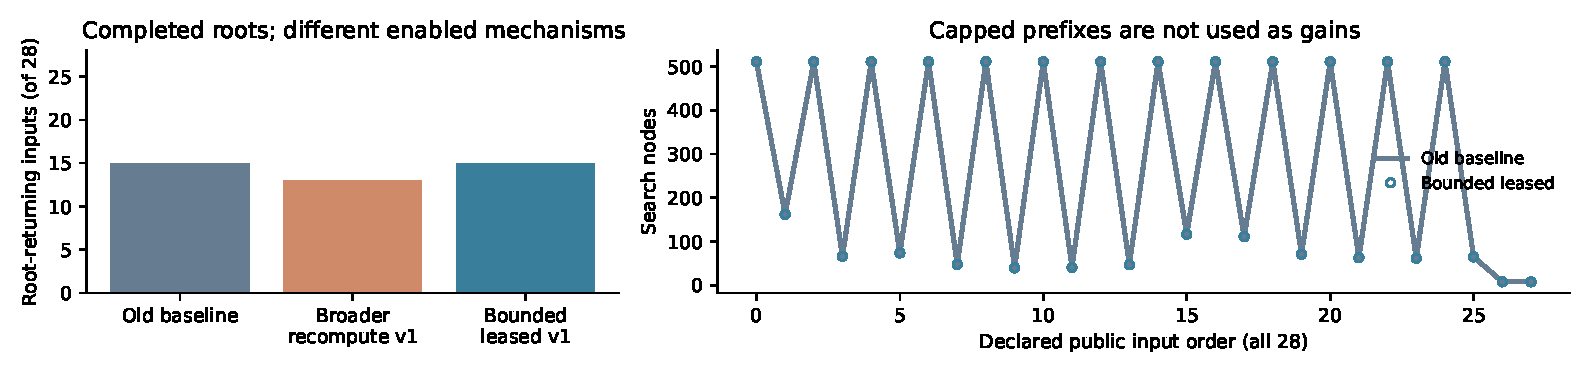
\includegraphics[width=\linewidth]{outcomes.pdf}\par
Recorded native counts only. The first panel includes the frozen previous
native reader values; the second retains all28 new inputs in declared order.
The separate synthetic conditional control changes3to2nodes; it is not a curve
result. No elapsed-time sample, uncertainty fit or scaling inference.
[pcc:unverified]

\textbf{Fixed interface and checks.} Disabled mode matches unchanged worklist
v1 answers, full decisions, counters and schedule on33systems. All returned
roots receive independent original-equation and native indexed-row/group
replay. Query arguments are public System, semantic roles, limits and mode;
never a scalar, witness, label, sign or point list. Replay tables are outside
the query and remain unpriced. Five Fp29 truth domains, labelled-unit/trace/root
mutations, forced caps and malformed refusals are retained. [pcc:unverified]

\textbf{Domains.} Toy p101/A95/h(17,12)/a17/q3/k8, arity2,13image targets,
distinct raw columns and aliases retained, identity columns excluded. Actual
$p=2^{255}-19$, A486662, $h_{new}=h_{old}^{213156431}$, a60824497/q1/k2,arity2.
This actual fixture has TWO columns. Huge original q213156431 systems receive
zero solver calls in this stage. [pcc:unverified]

\newpage
\begin{center}\Large Scope, accounting and source custody\end{center}
\textbf{Bounded slice.} At quiescence before a nonunique branch or Unsupported,
specialize original equations and select a connected slice of affine
residuals, in ascending equation order, at most32rows/64variables/256coefficient
entries. Sparse forward elimination carries original-equation weights.
Only a unit or nonzero constant affects search after coefficient checking.
Ignored rows make the slice incomplete. No full original-System copy or
dependency rebuild is performed; a bounded slice is recomputed at a new
quiescence, not maintained as a persistent incremental basis. [pcc:unverified]

\textbf{Accounting gate stays open.} Old limits remain1024nodes/depth128,
10million diagnostic events,64MiB cumulative modeled reservations,
4096variables/8192equations/32768terms/degree2. Extra1024pass/65536trace guards
and the slice bounds are finite. New component and in-query checker primitive
arithmetic, scans and modeled storage are charged before admission. Whole
cold parsing/serialization, replay, actual allocator/container overhead and
live-storage costs remain unpriced. No complete-cost, fastest-tool or speed
claim follows from these counters. [pcc:unverified]

\textbf{Frozen source.} Composite133inputs: unchanged98context plus35new
Rust/Cargo/request files. All36compiled bindings and six archive round-trips
match. No monolithic133archive. New21268-byte source delta SHA-256:\\
\texttt{d3f611b4faf005dfc72a679178d3f75b4c7c63aec6e36424b1079a1ac5cdf1df}.\par
Copied3323936-byte executable SHA-256:\\
\texttt{939476d96d8111aef1cb651d4d529f998d96c87c5a78d6b7dcbb1668022a8eba}.\par
Whole249-file/9258198-byte raw tree,34644-byte archive SHA-256:\\
\texttt{8b7339863e182f3ffdad1331c136f92e83a511b1202e56fd44c70cc2d9161df2}.\par
The separately copied qualifier is hashed before calls; build/pre-call/post-call
manifests are distinct. Native aggregates are computed in Rust. First compile
failure and initial source remain. Corrected release library/fmt/strict
all-target Clippy/build pass locally; no source edit after qualification.
See \path{leased-affine-v1/FROZEN.md} and \path{REPRODUCE.md}. [pcc:unverified]

\textbf{Prior art.} KB unavailable (MCP absent,wrapper127). Read previous
protocol/NEXT/native code and Soos, Nohl, Castelluccia,
\emph{Extending SAT Solvers to Cryptographic Problems}, section3.2 pp248--249:
\url{https://www.msoos.org/wordpress/wp-content/uploads/2011/03/Extending_SAT_2009.pdf}.
Boolean Gaussian/DPLL integration, explanations and restored state are prior
art, not a prime-field speed prediction or justification for tuning cutoffs.

\textbf{Next distinct hypothesis.} Bounded monomial-column elimination on
original quadratic rows could cancel nonlinear terms and expose affine units.
Check classical linearization/Macaulay prior art before a successor protocol;
retain all original constraints and certify weights. Original route-criteria
V3 yield/family/selection/rank/kernel/recovery and whole cold-work gates remain
open. No successor campaign is scheduled by the maintenance checker.
Canonical performance/exponent graphs and benchmarks stay unchanged: no
admitted performance datum is added. [pcc:unverified]

\textbf{Publication custody.} PR4475 merged externally during qualification.
Exact new subjects were transferred from checkpoint4f1a451157 to main2043bee6ae
without a native rerun; all98 predecessor inputs are present there. Its1279-row
ledger prefix is retained and only new unpublished claims are registered.
Seven older published registrations remain omitted upstream and archived
unchanged, never replayed. Older large-payload receipts remain separate
dependencies. Merge CI/reviews and signed standing are not inferred from
these producer checks. [pcc:unverified]
\end{document}
